% Options for packages loaded elsewhere
\PassOptionsToPackage{unicode}{hyperref}
\PassOptionsToPackage{hyphens}{url}
%
\documentclass[
  english,
  man]{apa6}
\usepackage{lmodern}
\usepackage{amssymb,amsmath}
\usepackage{ifxetex,ifluatex}
\ifnum 0\ifxetex 1\fi\ifluatex 1\fi=0 % if pdftex
  \usepackage[T1]{fontenc}
  \usepackage[utf8]{inputenc}
  \usepackage{textcomp} % provide euro and other symbols
\else % if luatex or xetex
  \usepackage{unicode-math}
  \defaultfontfeatures{Scale=MatchLowercase}
  \defaultfontfeatures[\rmfamily]{Ligatures=TeX,Scale=1}
\fi
% Use upquote if available, for straight quotes in verbatim environments
\IfFileExists{upquote.sty}{\usepackage{upquote}}{}
\IfFileExists{microtype.sty}{% use microtype if available
  \usepackage[]{microtype}
  \UseMicrotypeSet[protrusion]{basicmath} % disable protrusion for tt fonts
}{}
\makeatletter
\@ifundefined{KOMAClassName}{% if non-KOMA class
  \IfFileExists{parskip.sty}{%
    \usepackage{parskip}
  }{% else
    \setlength{\parindent}{0pt}
    \setlength{\parskip}{6pt plus 2pt minus 1pt}}
}{% if KOMA class
  \KOMAoptions{parskip=half}}
\makeatother
\usepackage{xcolor}
\IfFileExists{xurl.sty}{\usepackage{xurl}}{} % add URL line breaks if available
\IfFileExists{bookmark.sty}{\usepackage{bookmark}}{\usepackage{hyperref}}
\hypersetup{
  pdftitle={Relationship between social capital and election results},
  pdfauthor={Anisha Babu1, Hyeonjin Cha1, Diana DeWald1, \& Murat Kezer1},
  pdflang={en-EN},
  pdfkeywords={social capital, presidential elections},
  hidelinks,
  pdfcreator={LaTeX via pandoc}}
\urlstyle{same} % disable monospaced font for URLs
\usepackage{graphicx,grffile}
\makeatletter
\def\maxwidth{\ifdim\Gin@nat@width>\linewidth\linewidth\else\Gin@nat@width\fi}
\def\maxheight{\ifdim\Gin@nat@height>\textheight\textheight\else\Gin@nat@height\fi}
\makeatother
% Scale images if necessary, so that they will not overflow the page
% margins by default, and it is still possible to overwrite the defaults
% using explicit options in \includegraphics[width, height, ...]{}
\setkeys{Gin}{width=\maxwidth,height=\maxheight,keepaspectratio}
% Set default figure placement to htbp
\makeatletter
\def\fps@figure{htbp}
\makeatother
\setlength{\emergencystretch}{3em} % prevent overfull lines
\providecommand{\tightlist}{%
  \setlength{\itemsep}{0pt}\setlength{\parskip}{0pt}}
\setcounter{secnumdepth}{-\maxdimen} % remove section numbering
% Make \paragraph and \subparagraph free-standing
\ifx\paragraph\undefined\else
  \let\oldparagraph\paragraph
  \renewcommand{\paragraph}[1]{\oldparagraph{#1}\mbox{}}
\fi
\ifx\subparagraph\undefined\else
  \let\oldsubparagraph\subparagraph
  \renewcommand{\subparagraph}[1]{\oldsubparagraph{#1}\mbox{}}
\fi
% Manuscript styling
\usepackage{upgreek}
\captionsetup{font=singlespacing,justification=justified}

% Table formatting
\usepackage{longtable}
\usepackage{lscape}
% \usepackage[counterclockwise]{rotating}   % Landscape page setup for large tables
\usepackage{multirow}		% Table styling
\usepackage{tabularx}		% Control Column width
\usepackage[flushleft]{threeparttable}	% Allows for three part tables with a specified notes section
\usepackage{threeparttablex}            % Lets threeparttable work with longtable

% Create new environments so endfloat can handle them
% \newenvironment{ltable}
%   {\begin{landscape}\begin{center}\begin{threeparttable}}
%   {\end{threeparttable}\end{center}\end{landscape}}
\newenvironment{lltable}{\begin{landscape}\begin{center}\begin{ThreePartTable}}{\end{ThreePartTable}\end{center}\end{landscape}}

% Enables adjusting longtable caption width to table width
% Solution found at http://golatex.de/longtable-mit-caption-so-breit-wie-die-tabelle-t15767.html
\makeatletter
\newcommand\LastLTentrywidth{1em}
\newlength\longtablewidth
\setlength{\longtablewidth}{1in}
\newcommand{\getlongtablewidth}{\begingroup \ifcsname LT@\roman{LT@tables}\endcsname \global\longtablewidth=0pt \renewcommand{\LT@entry}[2]{\global\advance\longtablewidth by ##2\relax\gdef\LastLTentrywidth{##2}}\@nameuse{LT@\roman{LT@tables}} \fi \endgroup}

% \setlength{\parindent}{0.5in}
% \setlength{\parskip}{0pt plus 0pt minus 0pt}

% \usepackage{etoolbox}
\makeatletter
\patchcmd{\HyOrg@maketitle}
  {\section{\normalfont\normalsize\abstractname}}
  {\section*{\normalfont\normalsize\abstractname}}
  {}{\typeout{Failed to patch abstract.}}
\patchcmd{\HyOrg@maketitle}
  {\section{\protect\normalfont{\@title}}}
  {\section*{\protect\normalfont{\@title}}}
  {}{\typeout{Failed to patch title.}}
\makeatother
\shorttitle{U.S. Social Capital and Elections}
\keywords{social capital, presidential elections}
\DeclareDelayedFloatFlavor{ThreePartTable}{table}
\DeclareDelayedFloatFlavor{lltable}{table}
\DeclareDelayedFloatFlavor*{longtable}{table}
\makeatletter
\renewcommand{\efloat@iwrite}[1]{\immediate\expandafter\protected@write\csname efloat@post#1\endcsname{}}
\makeatother
\usepackage{csquotes}
\ifxetex
  % Load polyglossia as late as possible: uses bidi with RTL langages (e.g. Hebrew, Arabic)
  \usepackage{polyglossia}
  \setmainlanguage[]{english}
\else
  \usepackage[shorthands=off,main=english]{babel}
\fi
\usepackage[]{biblatex}
\addbibresource{r-references.bib}

\title{Relationship between social capital and election results}
\author{Anisha Babu\textsuperscript{1}, Hyeonjin Cha\textsuperscript{1}, Diana DeWald\textsuperscript{1}, \& Murat Kezer\textsuperscript{1}}
\date{}


\affiliation{\vspace{0.5cm}\textsuperscript{1} University of Oregon}

\abstract{
Social capital has been an important predictor of the U.S. presidential election results. However, previous studies conceptualizes social capital as a unidimensional construct. We argue that a multidimensional conceptualization of social capital will reveal patterns that will contribute to our understanding of social capital and its relationship with elections. In the present study, we first examine how social capital changes across years. Then, we investigate how different types of social capital (i.e., religion, civic, and labor) are associated with presidential election results across years. Social capital as a unidimensional construct was largely stable over the four time points used in this research (1997, 2005, 2009, and 2014). As such, it is unlikely that social capital has much impact on election results, as presidential winners typically alternate between the two major political parties. Moreover, our findings indicate that while an aggregate social capital negatively predicted democratic margin in the presidential elections, this was not the case when social capital was operationalized as a multidimensional construct. Therefore, future research should consider conceptualizing social capital as a construct comprised of a multitude of dimensions.
}



\begin{document}
\maketitle

\hypertarget{introduction}{%
\section{Introduction}\label{introduction}}

Social capital, a concept popularized in the late 20th century, describes a measure of connections among individuals within a society \autocite{putnam2000}. This measure is largely concerned with the cultural norms, interpersonal trust, and social connections that allow individuals to act together in the pursuit of common goals (Ibid). Social capital is often conceptualized by recording the presence of businesses, institutions, etc. in counties and the fluctuations in their presence over time. These institutions include religious organizations, civic associations, and sporting clubs, among others (see \enquote{data} section below for further details). Social science literature has previously examined the relationship between aggregate social capital and political involvement in European countries \autocites[e.g.,][]{morales2016}{jottier2012} as well as in the U.S. \autocite{la1998}.\\
More specifically, there are studies which implicate a relation between social capital and voting behavior in the 2016 presidential race \autocite[such as][]{lee2020}. Notably, \textcite{giuliano2020} found that the aggregate density of social capital at the county and individual levels in 2016 was negatively correlated with vote share for the republican candidate. However, relatively little is known about how specific (non-aggregate) sectors of social capital impacted presidential races in 2000, 2008, 2012, and 2016. To that end, we set out to explore the relation between social capital in U.S. counties from 1997-2014 and voting behavior during subsequent presidential races.

\hypertarget{methods}{%
\section{Methods}\label{methods}}

We report how we determined our sample size, all data exclusions (if any), all manipulations, and all measures in the study.

\hypertarget{data}{%
\subsection{Data}\label{data}}

The present study uses secondary datasets. First, \emph{The production of social capital in US counties constitutes the social capital data} \autocite{rupasingha2006}. Second, \emph{County Presidential Election Returns 2000-2016} \autocite{data6science} is used for presidential election results. Both datasets provide data on county level.\\
In the election data, we mainly used how many votes each political party received in each county as well as total number of votes in that election for a given county.\\
In the social capital data, we only selected the variables that were available in all time points. These variables were the number of bowling centers, civic and social associations, public golf courses, religious organizations, fitness and recreational sports centers, political organizations, professional organizations, business associations, labor organizations, and non-profit organizations. We also use the variables that indicate the population at county level, voter turnout, census response rate, and a social capital index.

\hypertarget{data-preparation}{%
\subsection{Data Preparation}\label{data-preparation}}

To prepare the data for analysis, we started with the election data as it is more comprehensive in terms of the number of counties. First, we selected the variables of interests. Then, we selected the election years (i.e., 2000, 2008, 2012, 2016) that match with social capital data. The name of the year variable was changed in a way that shows it is the year of election so that it is not mixed with the same year variable in social capital data. Next, we create new datasets for each presidential election we are interested in. These will be later merged with corresponding social capital data.\\
For each social capital dataset (i.e., 1997, 2005, 2009, 2014), we first added state code for some counties that do not readily contain that information. Then, we created two variables out of the area name such that we have different variables for county names and state codes. Then, we selected the relevant variables and cleaned the variable names. We only selected the variables that were available for all time points that we chose. Next, we created a year variable indicating when the data were collected.\\
Finally, we reorder the variables so that they are the same across datasets, and merged the four datasets to create one dataset that contains all of the data from each dataset.

\hypertarget{data-analysis}{%
\subsection{Data analysis}\label{data-analysis}}

First, we provide the descriptive statistics regarding election results in Table 1. Next, we visualize the distribution of the votes across U.S. Finally, we present several plots of our analyses and regression models in which elections results are predicted by an aggragate social capital variable as well as by different types of social capital.\\
We used R \autocite[Version 4.0.2;][]{R-base} and the R-packages \emph{broom} \autocite[Version 0.7.1;][]{R-broom}, \emph{corx} \autocite[Version 1.0.6.1;][]{R-corx}, \emph{dplyr} \autocite[Version 1.0.2;][]{R-dplyr}, \emph{forcats} \autocite[Version 0.5.0;][]{R-forcats}, \emph{ggplot2} \autocite[Version 3.3.2;][]{R-ggplot2}, \emph{ggpubr} \autocite[Version 0.4.0;][]{R-ggpubr}, \emph{here} \autocite[Version 0.1;][]{R-here}, \emph{janitor} \autocite[Version 2.0.1;][]{R-janitor}, \emph{kableExtra} \autocite[Version 1.3.1;][]{R-kableExtra}, \emph{knitr} \autocite[Version 1.30;][]{R-knitr}, \emph{magrittr} \autocite[Version 1.5;][]{R-magrittr}, \emph{papaja} \autocite[Version 0.1.0.9997;][]{R-papaja}, \emph{purrr} \autocite[Version 0.3.4;][]{R-purrr}, \emph{readr} \autocite[Version 1.3.1;][]{R-readr}, \emph{rio} \autocite[Version 0.5.16;][]{R-rio}, \emph{scales} \autocite[Version 1.1.1;][]{R-scales}, \emph{sjmisc} \autocite[Version 2.8.5;][]{R-sjmisc}, \emph{stringr} \autocite[Version 1.4.0;][]{R-stringr}, \emph{tibble} \autocite[Version 3.0.3;][]{R-tibble}, \emph{tidyr} \autocite[Version 1.1.2;][]{R-tidyr}, \emph{tidyverse} \autocite[Version 1.3.0;][]{R-tidyverse}, and \emph{usmap} \autocite[Version 0.5.1;][]{R-usmap} for all our analyses.

\hypertarget{visualization}{%
\subsection{Visualization}\label{visualization}}

We sought to answer our research questions with different visualizations. First, we explored how social capital changes over the four time points in our study (1997, 2005, 2009, and 2014). Next, we explored how U.S. presidential election results over the years (2000, 2008, 2012, and 2016) change depending on social capital in the preceding years. To supplement these analyses, we also consider geographic trends for election results and social capital across the U.S. and the state of Oregon.

\hypertarget{results}{%
\section{Results}\label{results}}

We start with a description of the presidential elections analyzed in this study, and continue with our main questions. Table 1 shows votes by candidate and year of election. Figure 1 visualizes the distributions of the votes in a U.S. map. Figure 2 shows the distribution of votes for the state of Oregon.

\begin{table}

\caption{(\#tab:descriptives table 1)A summary table for votes by candidate and year of election.}
\centering
\begin{tabular}[t]{c|c|c|c|c}
\hline
Year & Party & N & Mean Candidate Votes & SD Candidate Votes\\
\hline
2000 & Dem & 3107 & 16218 & 57150\\
\hline
2000 & Green & 3107 & -- & --\\
\hline
2000 & Rep & 3107 & 16049 & 38632\\
\hline
2000 & -- & 3107 & 339 & 954\\
\hline
2008 & Dem & 3108 & 22157 & 76972\\
\hline
2008 & Rep & 3108 & 19167 & 44840\\
\hline
2008 & -- & 3108 & 577 & 1848\\
\hline
2012 & Dem & 3108 & 20974 & 73998\\
\hline
2012 & Rep & 3108 & 19409 & 44596\\
\hline
2012 & -- & 3108 & 838 & 2952\\
\hline
2016 & Dem & 3115 & 21071 & 80496\\
\hline
2016 & Rep & 3115 & 20160 & 43157\\
\hline
2016 & -- & 3115 & 2449 & 7509\\
\hline
\multicolumn{5}{l}{\rule{0pt}{1em}\textit{Note: } N = total number of counties in the US reporting data.}\\
\end{tabular}
\end{table}

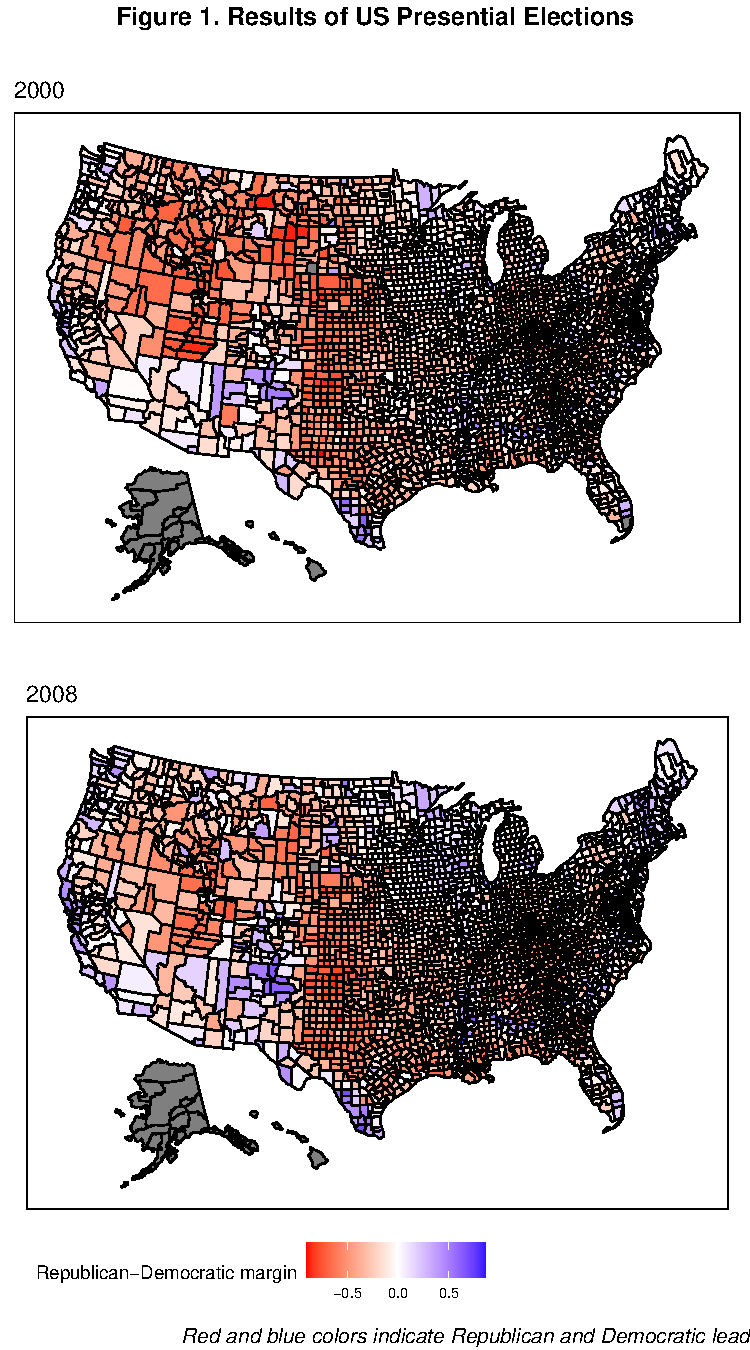
\includegraphics{Script_files/figure-latex/visualization US election results-1.pdf} 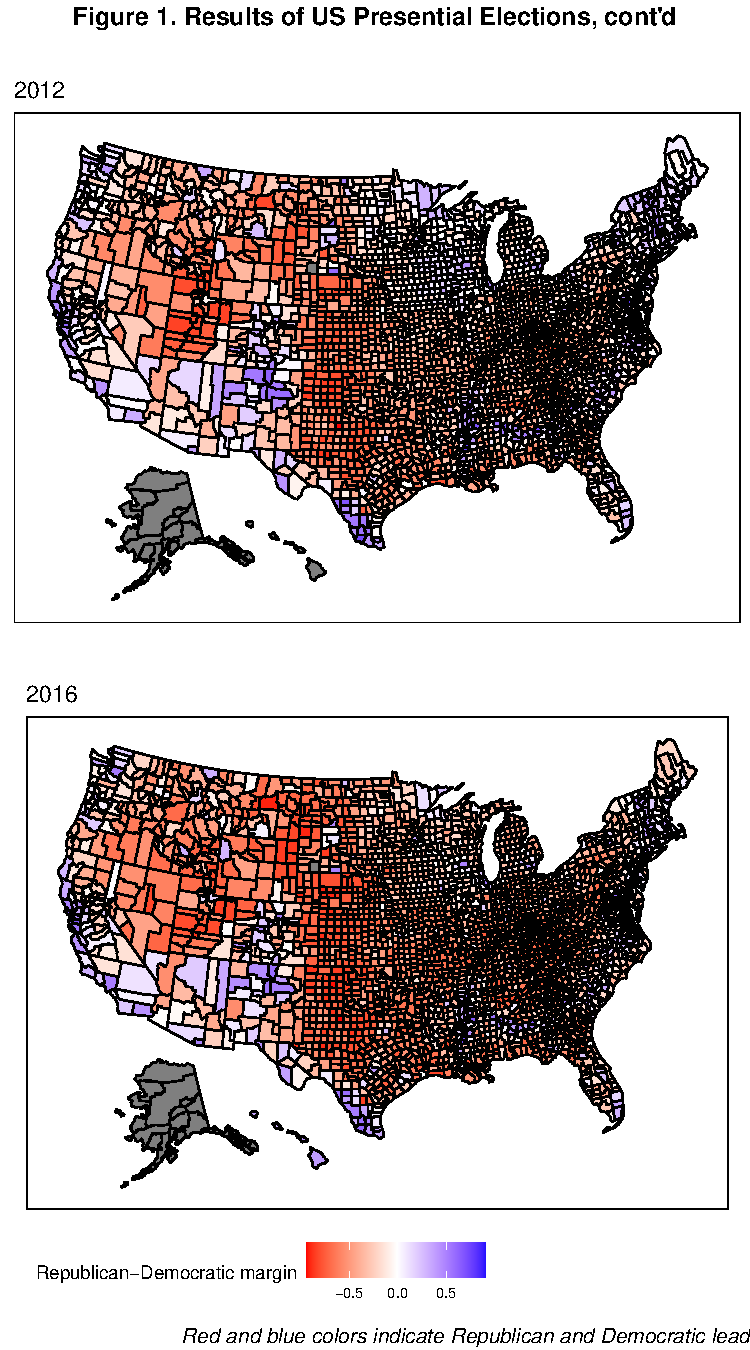
\includegraphics{Script_files/figure-latex/visualization US election results-2.pdf}

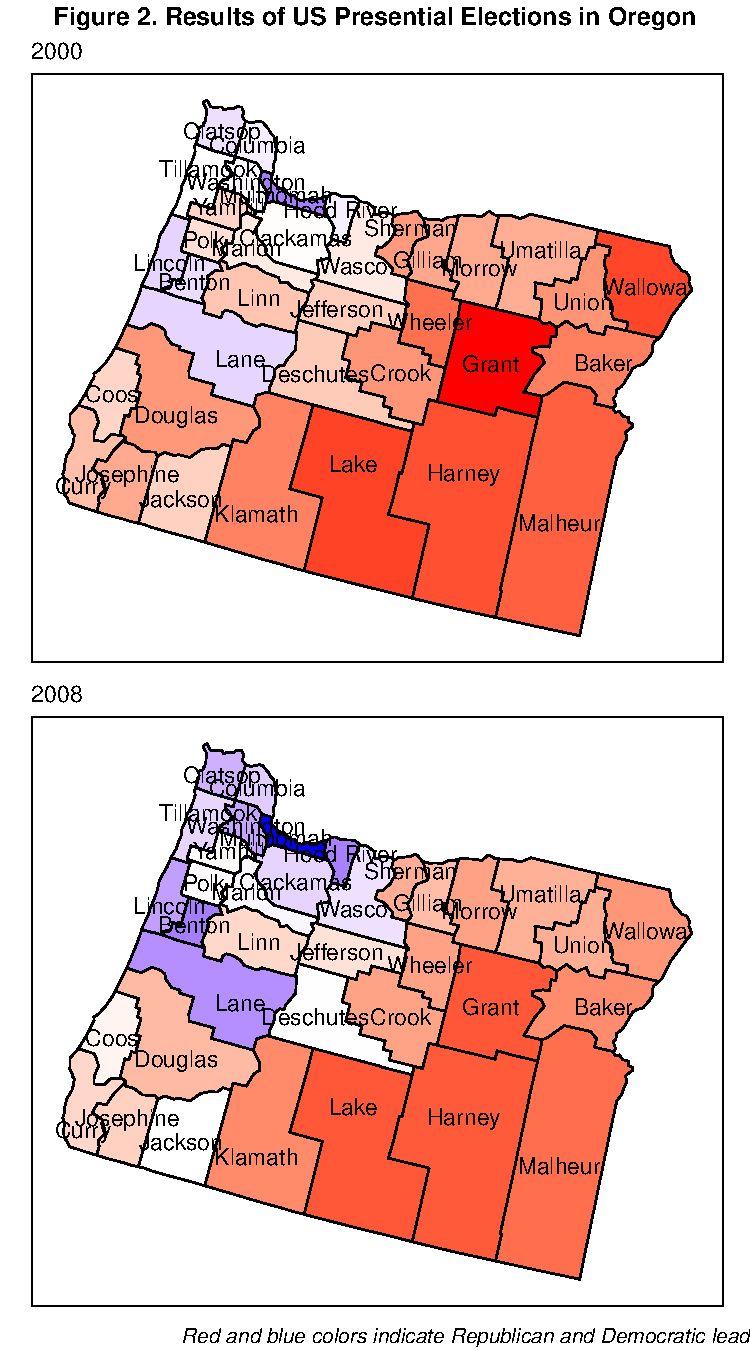
\includegraphics{Script_files/figure-latex/visualization Oregon election results-1.pdf} 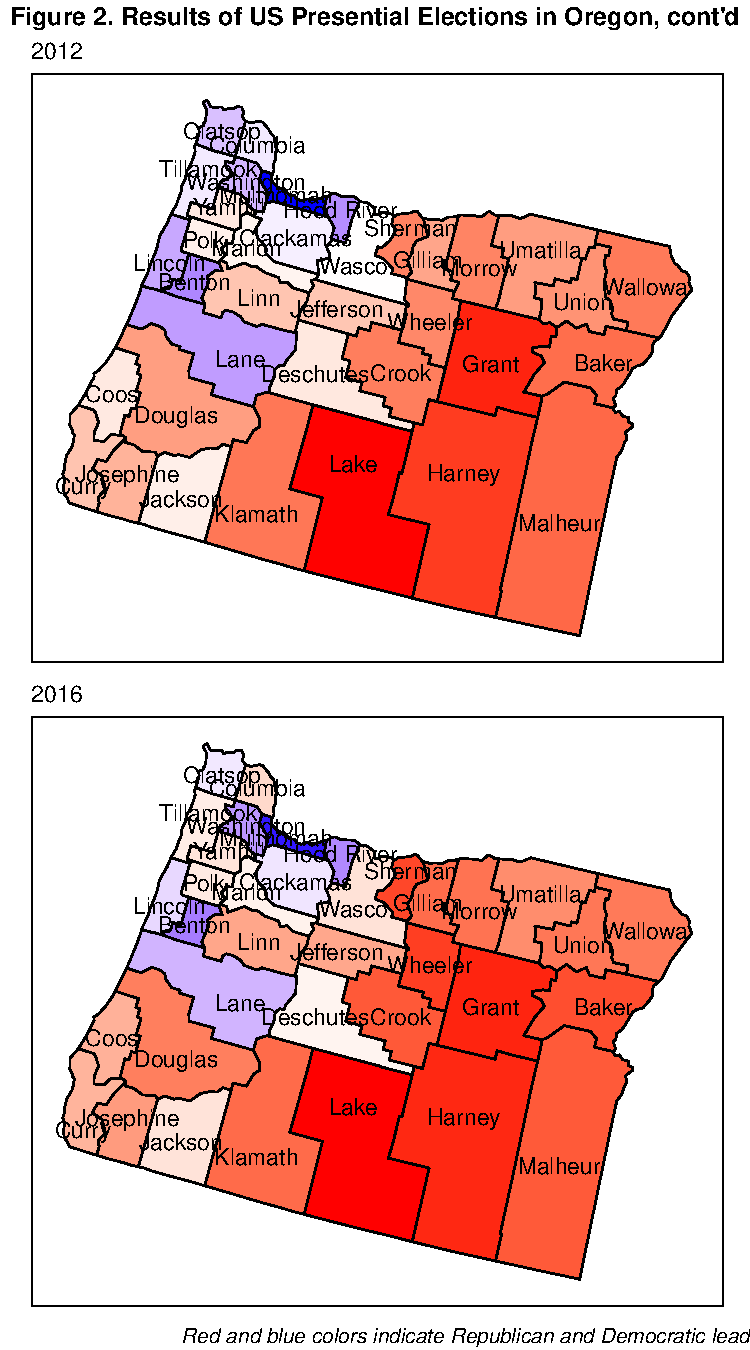
\includegraphics{Script_files/figure-latex/visualization Oregon election results-2.pdf}

\hypertarget{how-does-social-capital-change-over-time}{%
\subsection{How does social capital change over time?}\label{how-does-social-capital-change-over-time}}

We considered how social capital changes over time. To do so, we first created an \enquote{aggregate social capital} variable for each state. This variable represents the sum of all social capital types (bowling, civic, golf, religion, sport, political, professional, business, and labor) across all counties in a given state. To account for differences in state population, this aggregate variable was divided by the total population.

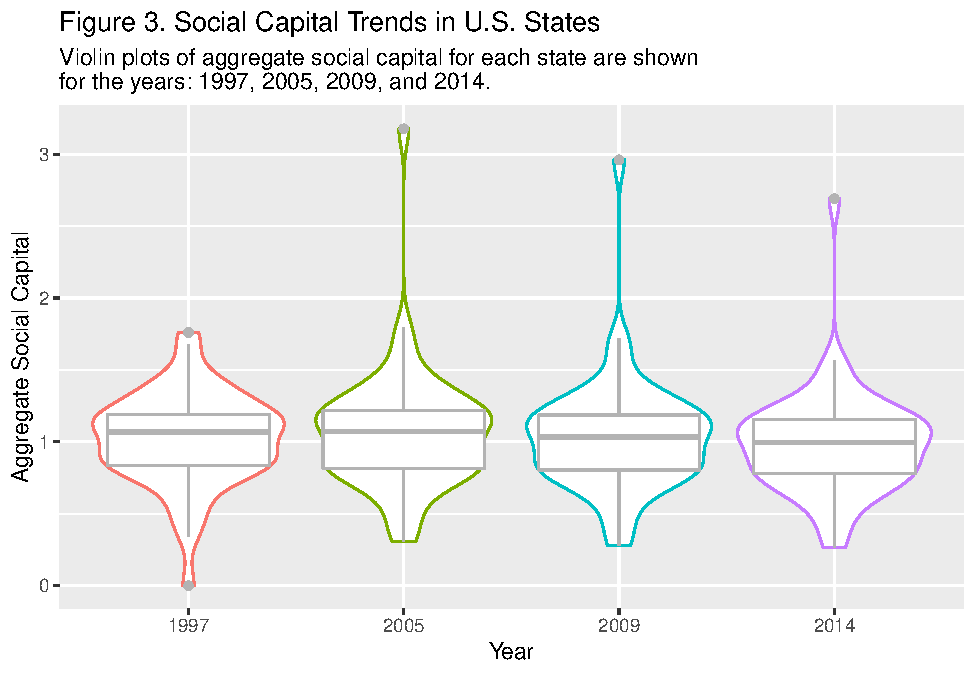
\includegraphics{Script_files/figure-latex/violin-1.pdf}
Figure 3: Violin plots of aggregate social capital for each state are shown for the years: 1997, 2005, 2009, and 2014. Overlaid are boxplots representing each distribution's minimum, maximum, medium, and first and third quartiles. Aggregate social capital variables (described above) were multiplied by 1000 to avoid small decimal values and improve readability.

This graph shows relatively consistent aggregate social capital over the years. It is important to note that the lower outlier in the year 1997, and the upper outliers in years 2005, 2009, and 2014 are values for Washington, D.C. Without this value, distributions would be nearly identical across all time points.\\
As a secondary measure of aggregate social capital, we considered the provided values from our dataset. These provided values summed all types of social capital, divided by population per 10,000, and divided by 10 (1st factor). These values were used to visualize geographic trends in social capital.\\
GEOGRAPHICAL TRENDS - MAY NEED MAP PLOTS HERE, OTHERWISE REMOVE ABOVE PARAGRAPH

We also considered how specific types of social capital change over time. As such, we focused on religion, civic, and labor types of social capital trends over time.

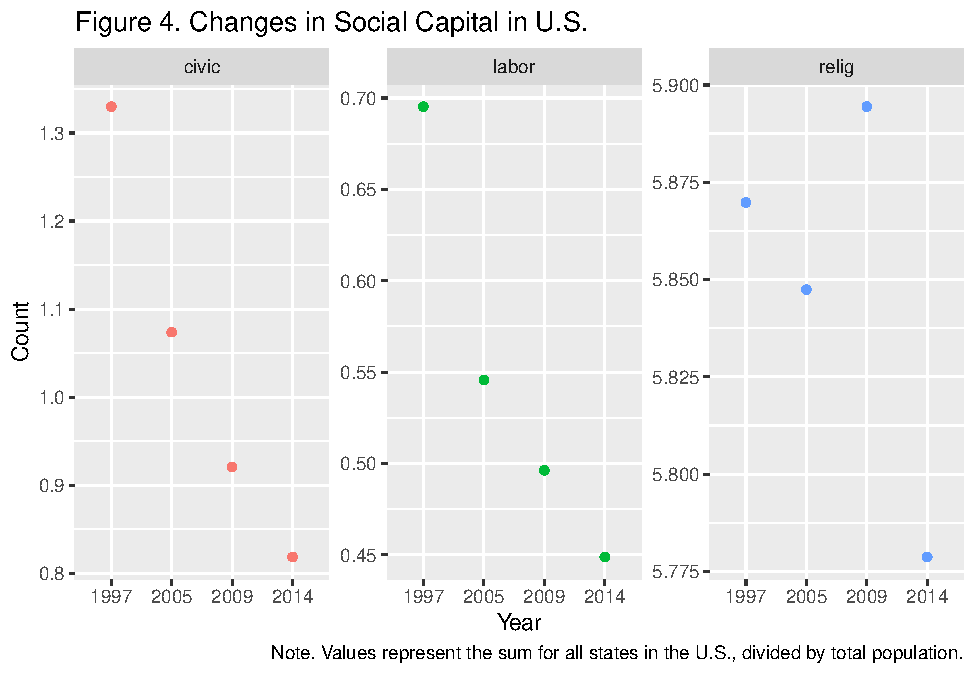
\includegraphics{Script_files/figure-latex/scatterplot-1.pdf}
Figure 4: These scatterplots show the changes in religion, civic, and labor social capital across years.

We then explored geographic trends for specific types of social capital. Figures 5a-7b visualize the distribution of the specific types of social capital on a U.S. map.

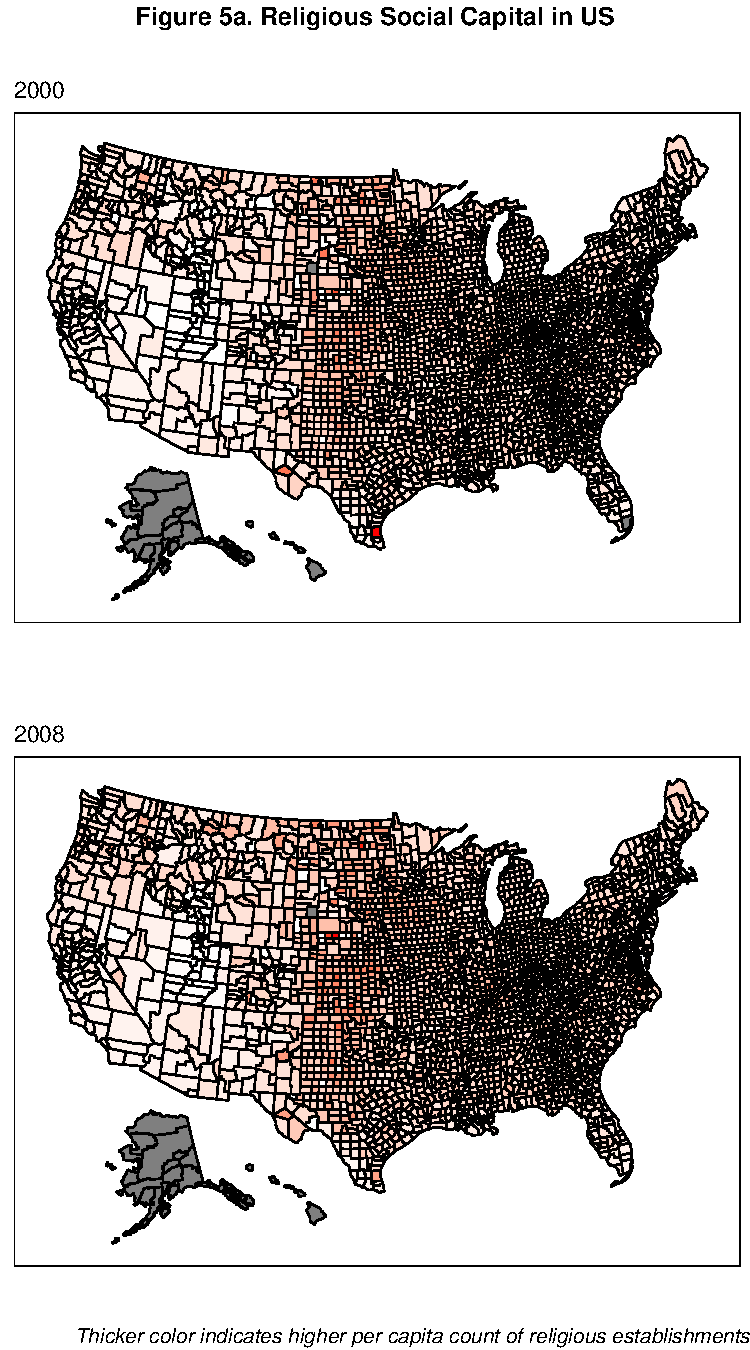
\includegraphics{Script_files/figure-latex/visualization religious capital US map-1.pdf} 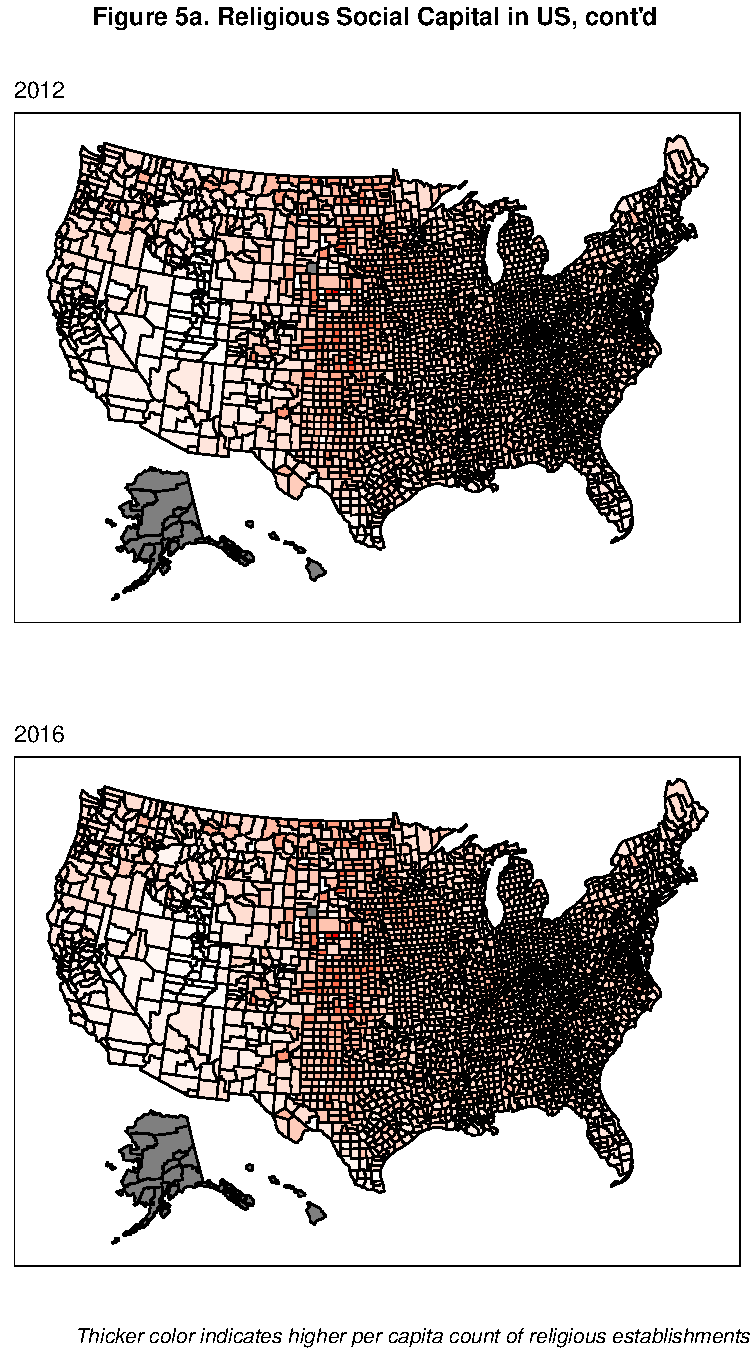
\includegraphics{Script_files/figure-latex/visualization religious capital US map-2.pdf} 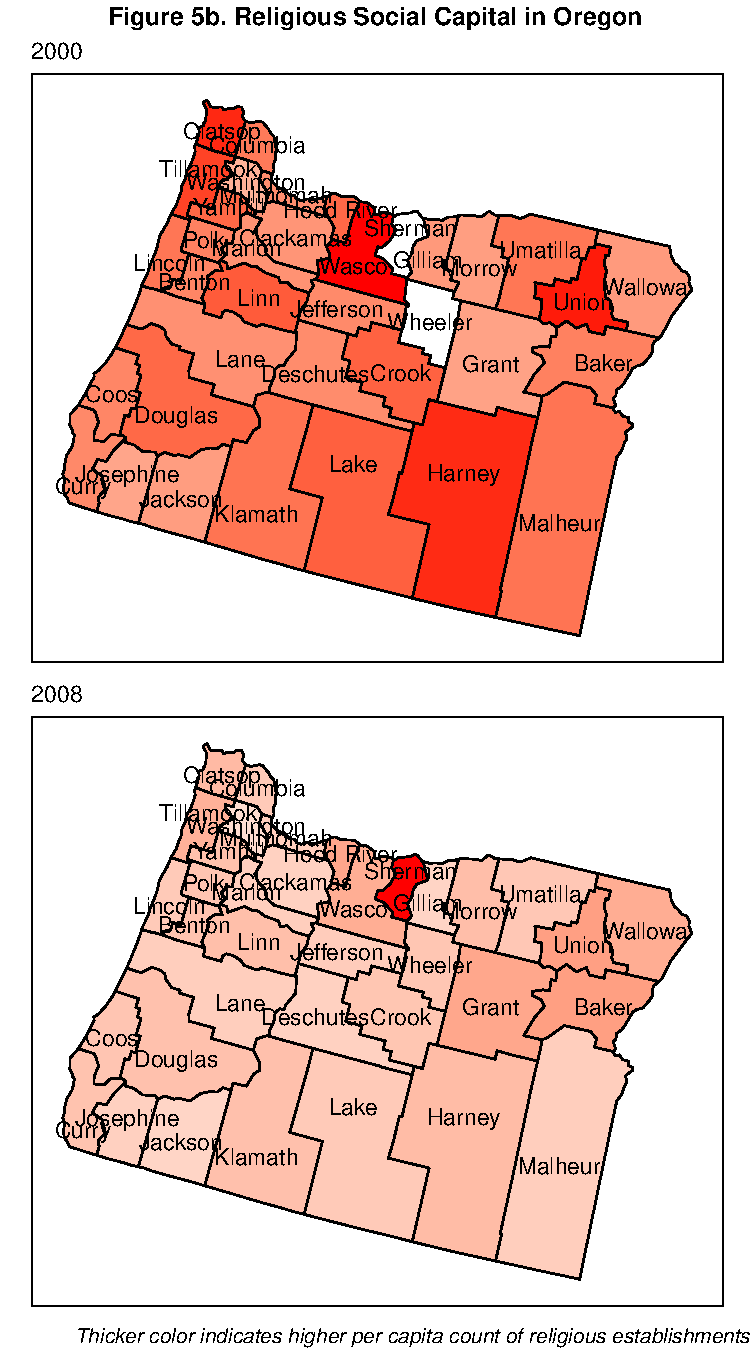
\includegraphics{Script_files/figure-latex/visualization religious capital US map-3.pdf} 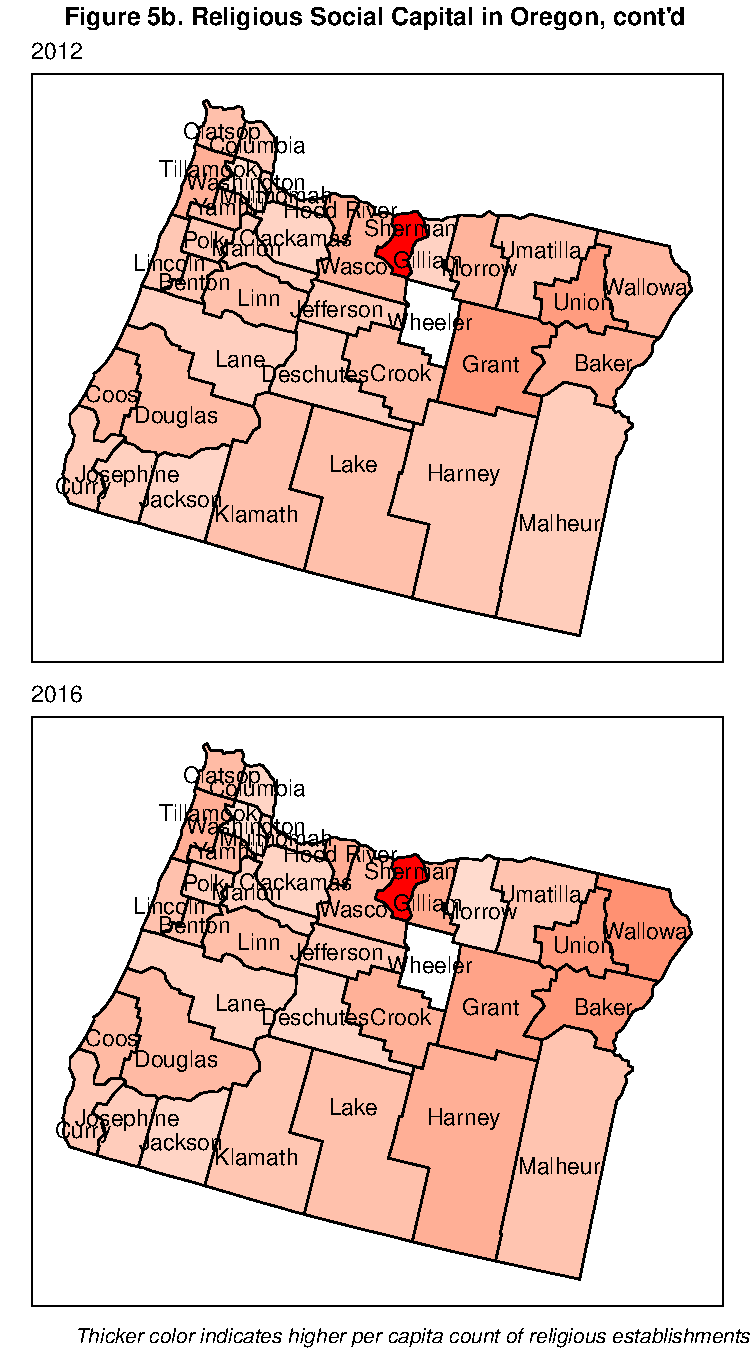
\includegraphics{Script_files/figure-latex/visualization religious capital US map-4.pdf}

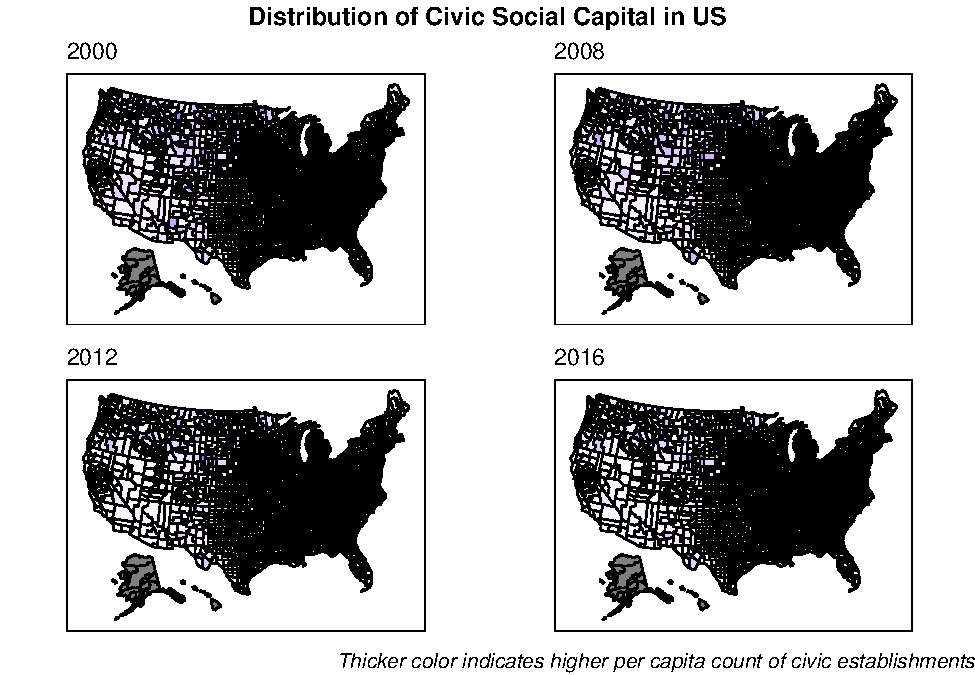
\includegraphics{Script_files/figure-latex/visualization civic social capital maps-1.pdf} 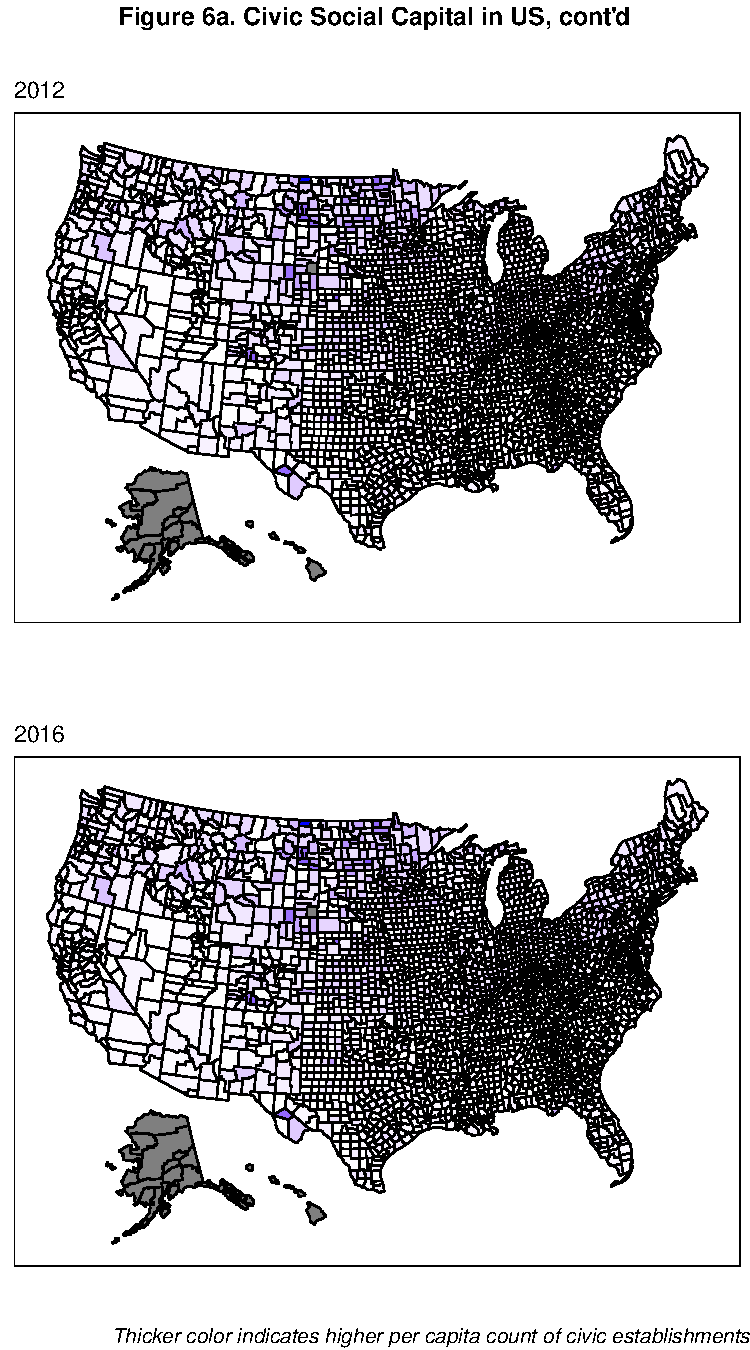
\includegraphics{Script_files/figure-latex/visualization civic social capital maps-2.pdf} 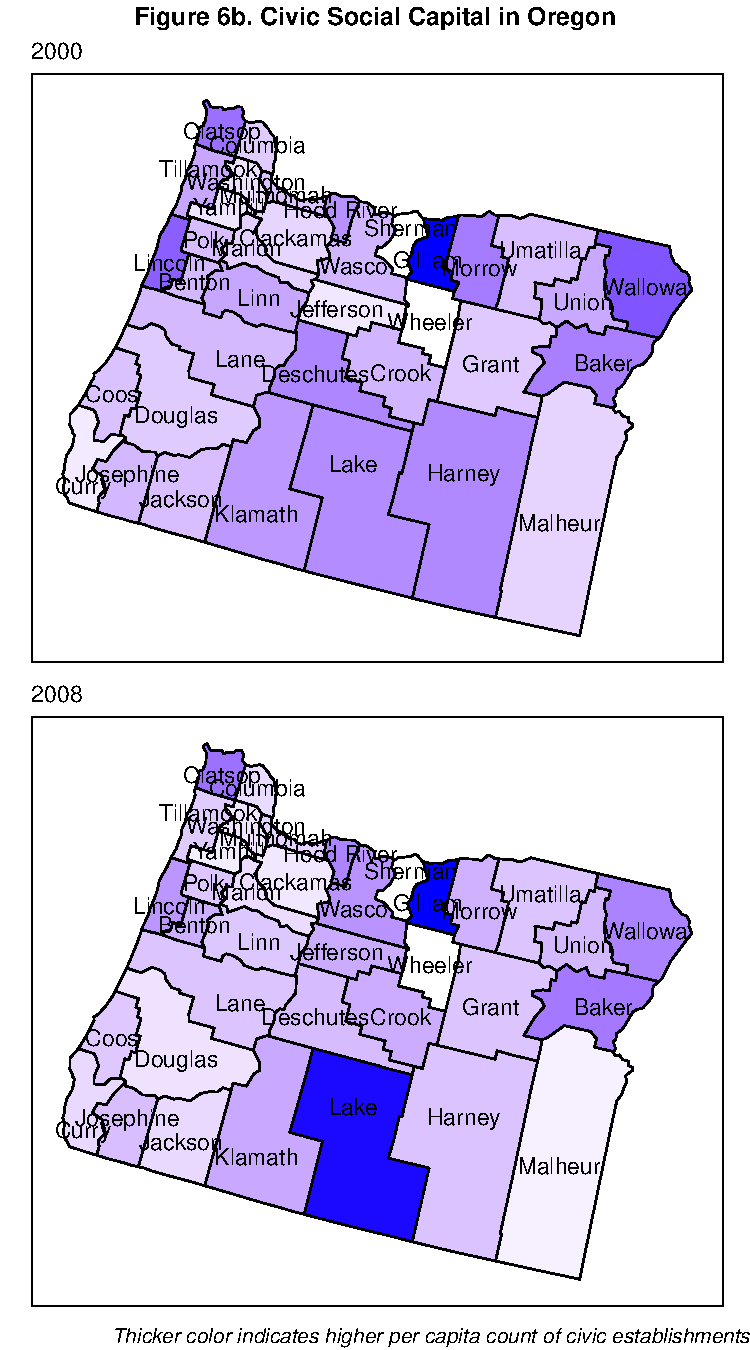
\includegraphics{Script_files/figure-latex/visualization civic social capital maps-3.pdf} 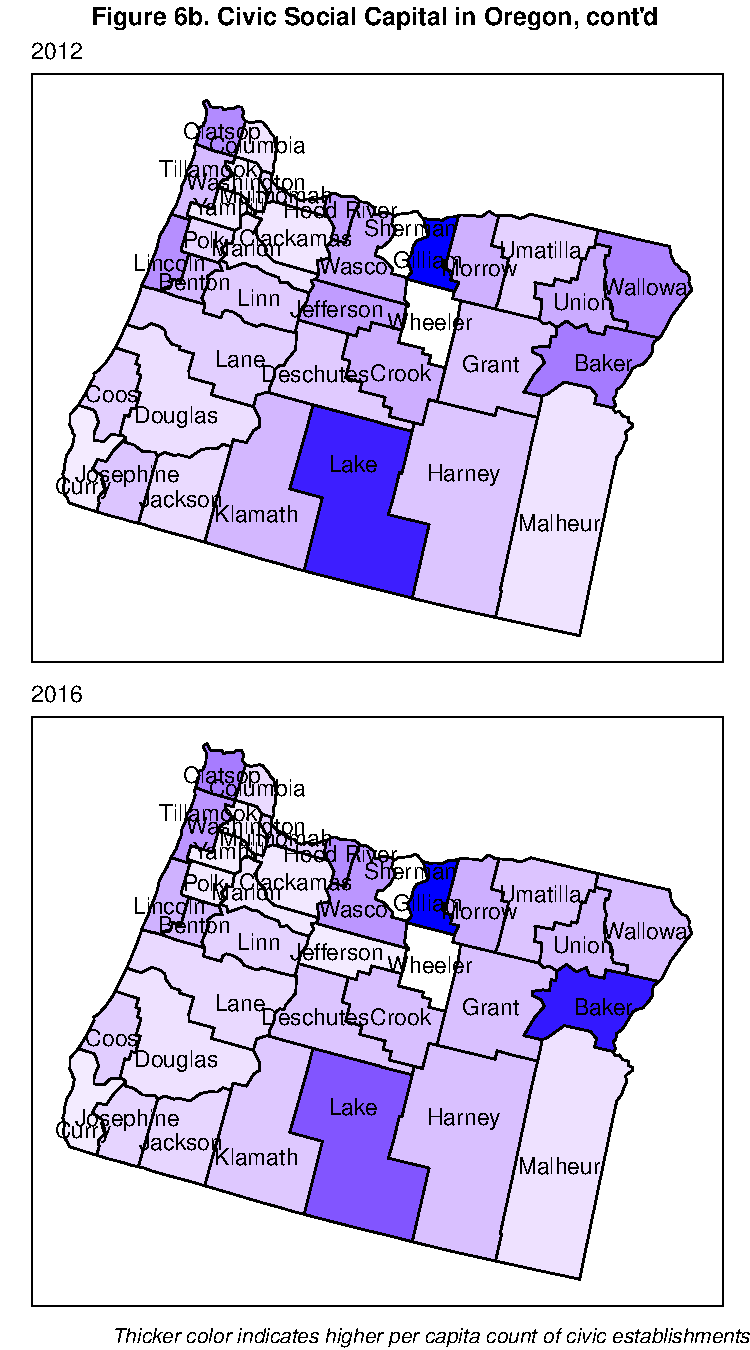
\includegraphics{Script_files/figure-latex/visualization civic social capital maps-4.pdf}

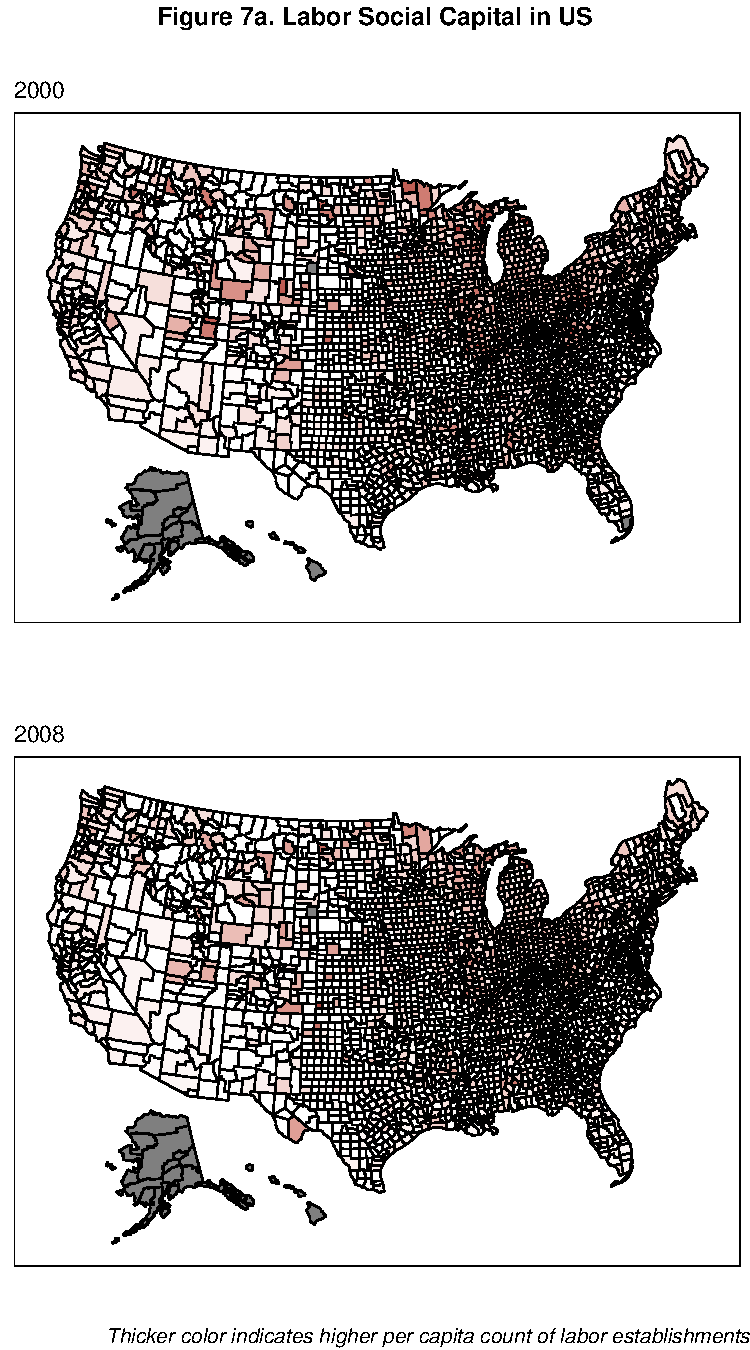
\includegraphics{Script_files/figure-latex/visualization labor social capital maps-1.pdf} 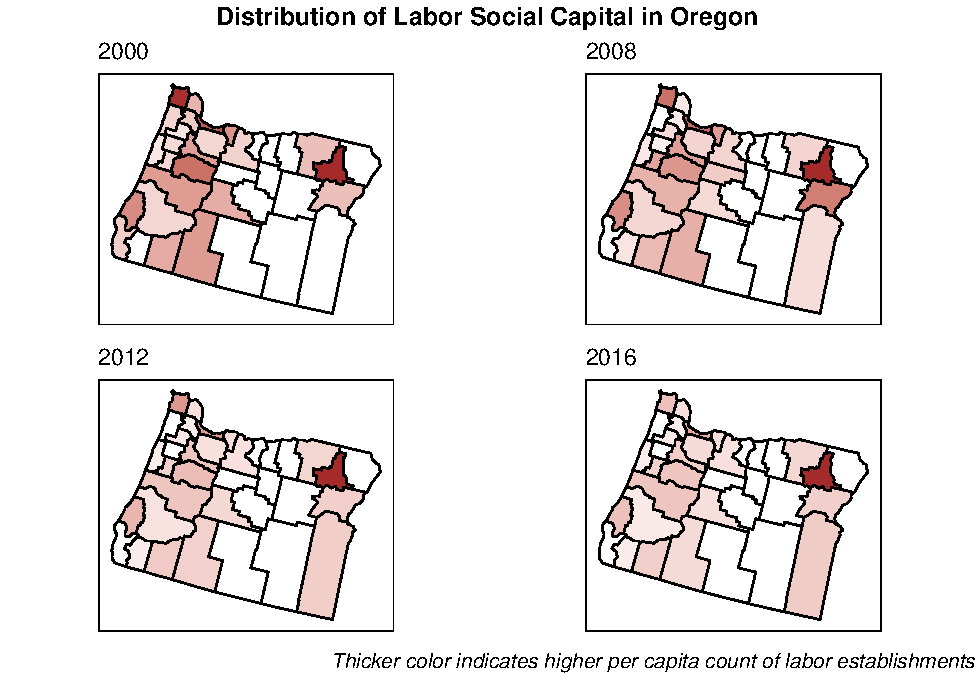
\includegraphics{Script_files/figure-latex/visualization labor social capital maps-2.pdf} 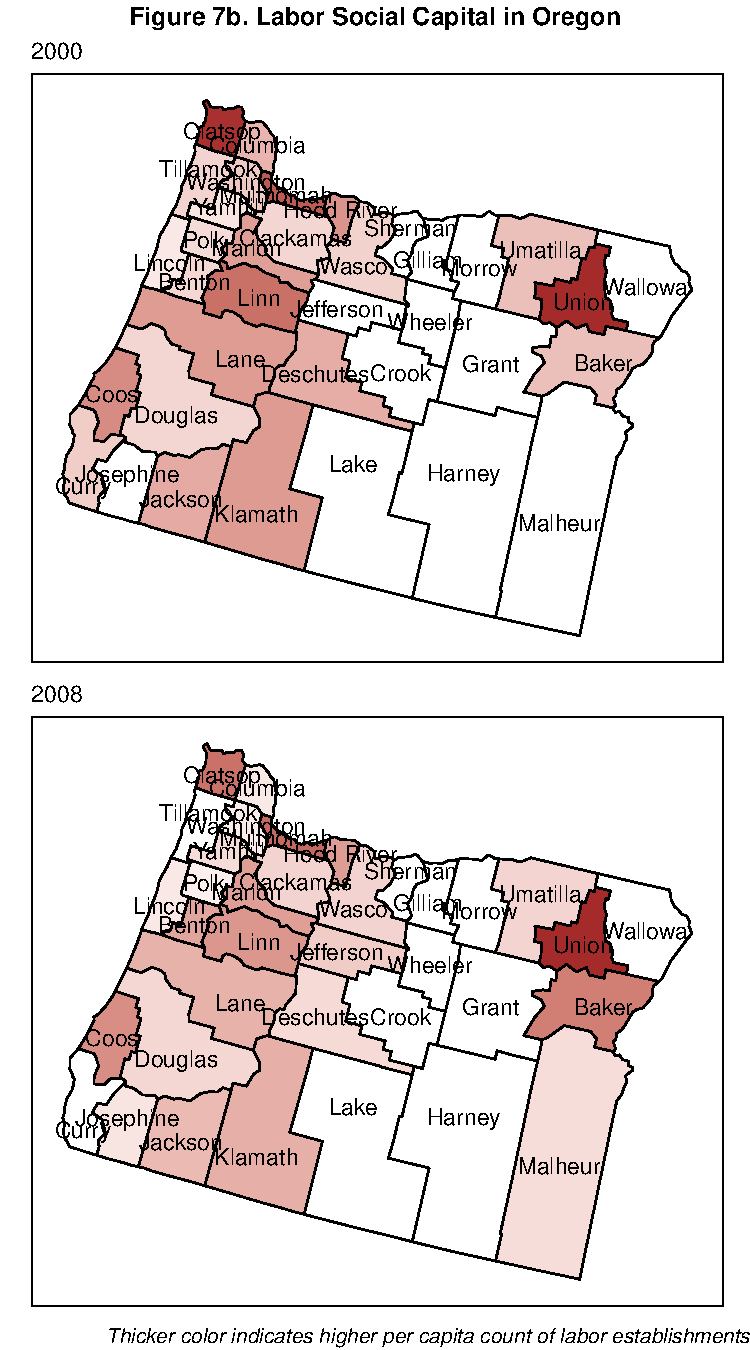
\includegraphics{Script_files/figure-latex/visualization labor social capital maps-3.pdf} 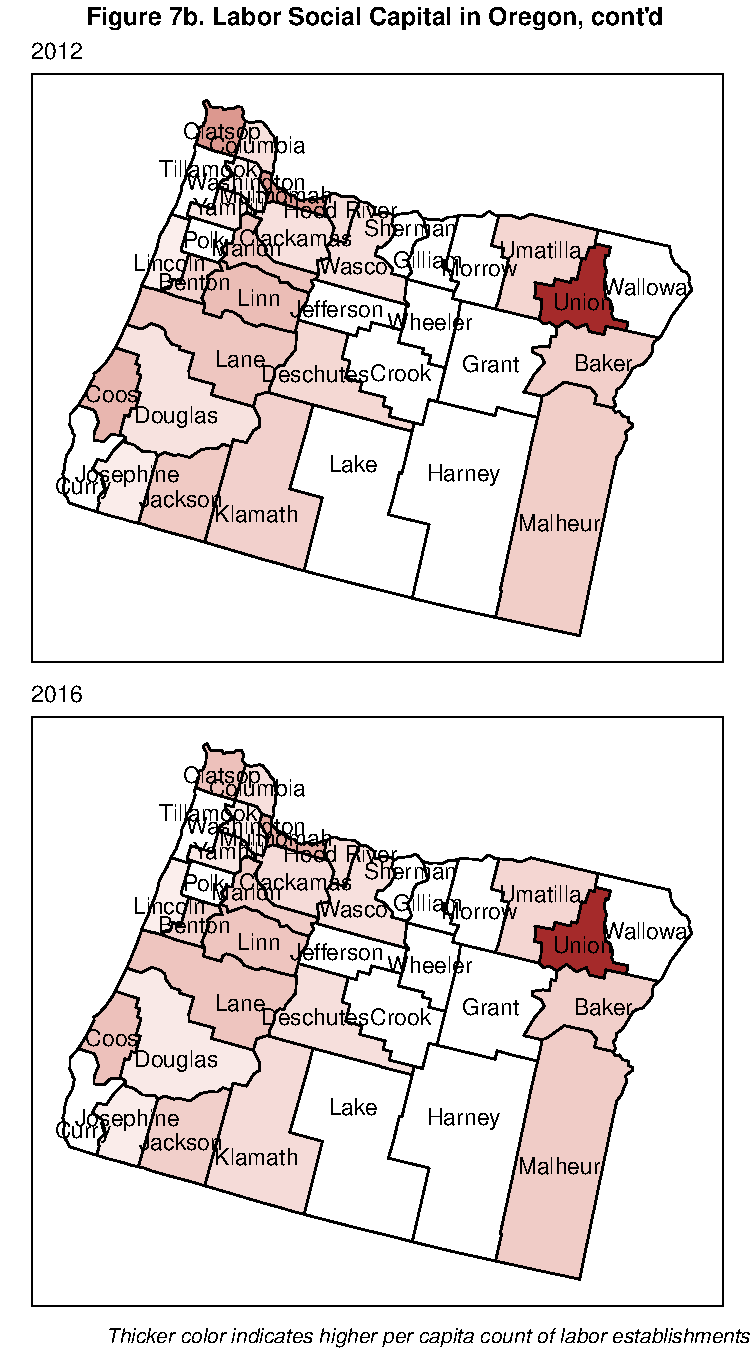
\includegraphics{Script_files/figure-latex/visualization labor social capital maps-4.pdf}

\hypertarget{relationship-between-social-capital-and-election-results}{%
\subsection{Relationship between social capital and election results}\label{relationship-between-social-capital-and-election-results}}

Finally, we considered the relationship between social capital and election results. The figure below shows how proportion of votes for the two major parties relates to aggregate social capital in the preceding years.\\
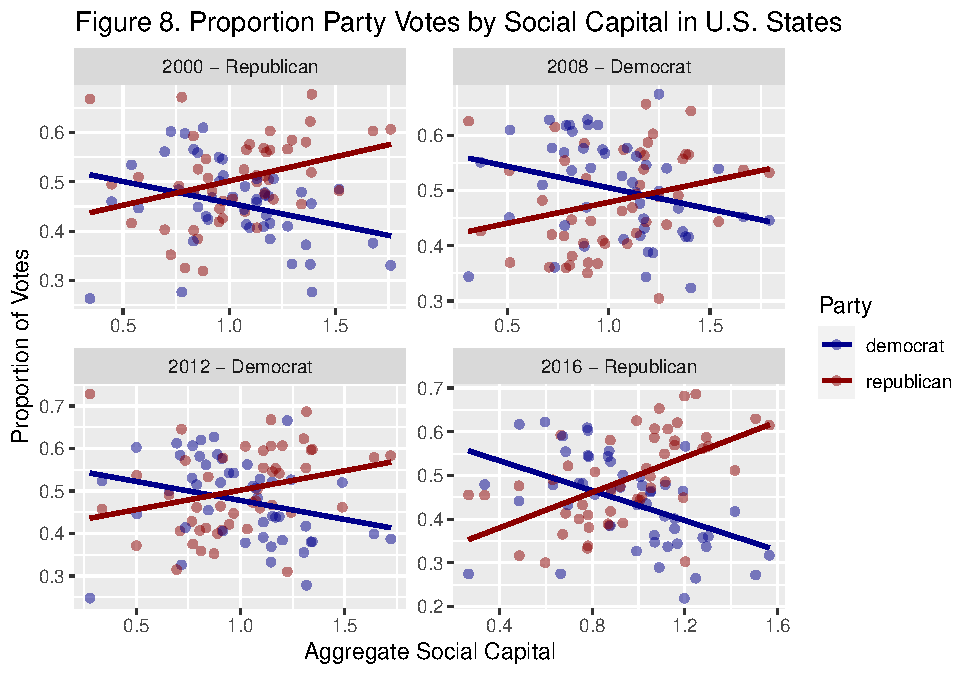
\includegraphics{Script_files/figure-latex/scatter and line-1.pdf}
Figure 8: This graph shows the relationship between aggregate social capital (same values as Figure 1) and proportion of votes for political parties (democrat in blue, republican in red) over the years.

This set of plots reveals trends between aggregate social capital and proportion of political party votes. Data for Washington, D.C. was not included in these plots as it was an outlier. This figure reveals that as aggregate social capital increases, proportion of democrat votes decreases and proportion of republican votes increases.\\
Next, to test this relationship, we regressed democratic margin on aggregate social capital. Table 2 displays the results. Across all election years, social capital negatively predicts democratic margin, all ps \textless{} .05. In the 2012 \& 2016 elections, this relationship seems to be stronger. However, this relationship is inconsistent with the theoretical view that suggests a positive relationship between social capital and democratic margin \autocite[e.g.,][]{giuliano2020}. Therefore, we look at how different types of social capital predict democratic margin. Table 3 presents the results. Consistent with our earlier finding, religious social capital is also negatively associated with democratic margin across elections. However, we found that civic social capital is positively associated with democratic margin in all elections except for the 2000 election. In a similar vein, labor social capital has a positive and strong relationship with democratic margin across all elections.

\begin{table}

\caption{\label{tab:regression}Table 2. Democratic Margin Predicted by Aggregate Social Capital}
\centering
\begin{tabular}[t]{r|r|r|r}
\hline
Term & B & SE & p\\
\hline
\multicolumn{4}{l}{\textbf{2000 Election}}\\
\hline
\hspace{1em}Intercept & -0.08 & 0.01 & <0.05\\
\hline
\hspace{1em}Social\_Capital\_(aggregate) & -0.07 & 0.01 & \vphantom{1} <0.05\\
\hline
\multicolumn{4}{l}{\textbf{2008 Election}}\\
\hline
\hspace{1em}Intercept & -0.07 & 0.01 & <0.05\\
\hline
\hspace{1em}Social\_Capital\_(aggregate) & -0.07 & 0.01 & <0.05\\
\hline
\multicolumn{4}{l}{\textbf{2012 Election}}\\
\hline
\hspace{1em}Intercept & -0.10 & 0.01 & <0.05\\
\hline
\hspace{1em}Social\_Capital\_(aggregate) & -0.09 & 0.01 & <0.05\\
\hline
\multicolumn{4}{l}{\textbf{2016 Election}}\\
\hline
\hspace{1em}Intercept & -0.16 & 0.01 & <0.05\\
\hline
\hspace{1em}Social\_Capital\_(aggregate) & -0.13 & 0.01 & <0.05\\
\hline
\end{tabular}
\end{table}
\begin{table}

\caption{\label{tab:regression2}Table 3. Correlation between social capital variables (2014) and democratic margin (2016)}
\centering
\begin{tabular}[t]{l|c|c|c|c|c|c|c|c|c|c|c}
\hline
  & 1 & 2 & 3 & 4 & 5 & 6 & 7 & 8 & 9 & 10 & 11\\
\hline
1. Bowling & - &  &  &  &  &  &  &  &  &  & \\
\hline
2. Civic & .16* & - &  &  &  &  &  &  &  &  & \\
\hline
3. Golf & .18* & .17* & - &  &  &  &  &  &  &  & \\
\hline
4. Religious & .18* & .25* & .35* & - &  &  &  &  &  &  & \\
\hline
5. Sport & -.01 & .00 & -.02 & .00 & - &  &  &  &  &  & \\
\hline
6. Political & -.03 & .00 & -.03 & .00 & .01 & - &  &  &  &  & \\
\hline
7. Professional & -.01 & .08* & -.04* & -.03 & .02 & .20* & - &  &  &  & \\
\hline
8. Business & .10* & .14* & .14* & .31* & -.02 & .09* & .16* & - &  &  & \\
\hline
9. Labor & .01 & .13* & -.03 & -.05* & .02 & .05* & .11* & -.02 & - &  & \\
\hline
10. NonProfit & .22* & .35* & .28* & .37* & .02 & .09* & .14* & .33* & .00 & - & \\
\hline
11. Social Capital Index & .29* & .46* & .43* & .68* & .03 & .09* & .13* & .44* & .03 & .85* & -\\
\hline
12. Democratic Margin & -.09* & -.04* & -.14* & -.33* & .02 & .09* & .19* & -.09* & .13* & -.07* & -.14*\\
\hline
\multicolumn{12}{l}{\rule{0pt}{1em}\textit{Note: } * p < .05; ** p < .01; *** p < .001}\\
\end{tabular}
\end{table}

\begin{table}

\caption{\label{tab:regression2}Table X. Correlation between social capital variables (2009) and democratic margin (2012)}
\centering
\begin{tabular}[t]{l|c|c|c|c|c|c|c|c|c|c|c}
\hline
  & 1 & 2 & 3 & 4 & 5 & 6 & 7 & 8 & 9 & 10 & 11\\
\hline
1. Bowling & - &  &  &  &  &  &  &  &  &  & \\
\hline
2. Civic & .21* & - &  &  &  &  &  &  &  &  & \\
\hline
3. Golf & .23* & .18* & - &  &  &  &  &  &  &  & \\
\hline
4. Religious & .23* & .23* & .42* & - &  &  &  &  &  &  & \\
\hline
5. Sport & -.02 & -.01 & -.02 & .00 & - &  &  &  &  &  & \\
\hline
6. Political & .00 & .05* & -.04* & -.01 & .01 & - &  &  &  &  & \\
\hline
7. Professional & .06* & .05* & -.04* & -.01 & .01 & .24* & - &  &  &  & \\
\hline
8. Business & .12* & .21* & .17* & .26* & -.02 & .15* & .22* & - &  &  & \\
\hline
9. Labor & .04* & .13* & -.05* & -.03 & .01 & .06* & .11* & -.04* & - &  & \\
\hline
10. NonProfit & .29* & .38* & .33* & .41* & .01 & .09* & .16* & .33* & .01 & - & \\
\hline
11. Social Capital Index & .36* & .47* & .48* & .65* & .03 & .10* & .16* & .41* & .05* & .86* & -\\
\hline
12. Democratic Margin & -.05* & .02 & -.10* & -.27* & .02 & .06* & .12* & -.12* & .19* & -.05* & -.08*\\
\hline
\multicolumn{12}{l}{\rule{0pt}{1em}\textit{Note: } * p < .05; ** p < .01; *** p < .001}\\
\end{tabular}
\end{table}

\begin{table}

\caption{\label{tab:regression2}Table X. Correlation between social capital variables (2005) and democratic margin (2008)}
\centering
\begin{tabular}[t]{l|c|c|c|c|c|c|c|c|c|c|c}
\hline
  & 1 & 2 & 3 & 4 & 5 & 6 & 7 & 8 & 9 & 10 & 11\\
\hline
1. Bowling & - &  &  &  &  &  &  &  &  &  & \\
\hline
2. Civic & .29* & - &  &  &  &  &  &  &  &  & \\
\hline
3. Golf & .23* & .18* & - &  &  &  &  &  &  &  & \\
\hline
4. Religious & .22* & .24* & .34* & - &  &  &  &  &  &  & \\
\hline
5. Sport & -.04* & .04* & -.05* & -.09* & - &  &  &  &  &  & \\
\hline
6. Political & -.02 & .04* & -.05* & -.01 & .05* & - &  &  &  &  & \\
\hline
7. Professional & .02 & .12* & -.03 & .03 & .12* & .21* & - &  &  &  & \\
\hline
8. Business & .11* & .13* & .16* & .26* & -.01 & .12* & .17* & - &  &  & \\
\hline
9. Labor & .02 & .15* & -.04* & -.01 & .14* & .12* & .10* & -.02 & - &  & \\
\hline
10. NonProfit & .30* & .37* & .29* & .40* & .02 & .06* & .18* & .30* & .02 & - & \\
\hline
11. Social Capital Index & .39* & .48* & .42* & .63* & .01 & .07* & .18* & .35* & .11* & .81* & -\\
\hline
12. Democratic Margin & -.04* & .08* & -.07* & -.23* & .14* & .06* & .12* & -.14* & .23* & -.03 & -.05*\\
\hline
\multicolumn{12}{l}{\rule{0pt}{1em}\textit{Note: } * p < .05; ** p < .01; *** p < .001}\\
\end{tabular}
\end{table}

\begin{table}

\caption{\label{tab:regression2}Table X. Correlation between social capital variables (1997) and democratic margin (2000)}
\centering
\begin{tabular}[t]{l|c|c|c|c|c|c|c|c|c|c|c}
\hline
  & 1 & 2 & 3 & 4 & 5 & 6 & 7 & 8 & 9 & 10 & 11\\
\hline
1. Bowling & - &  &  &  &  &  &  &  &  &  & \\
\hline
2. Civic & .25* & - &  &  &  &  &  &  &  &  & \\
\hline
3. Golf & .22* & .18* & - &  &  &  &  &  &  &  & \\
\hline
4. Religious & .23* & .21* & .17* & - &  &  &  &  &  &  & \\
\hline
5. Sport & -.01 & .04* & .01 & .01 & - &  &  &  &  &  & \\
\hline
6. Political & -.02 & .05* & -.01 & -.06* & .04* & - &  &  &  &  & \\
\hline
7. Professional & .03 & .12* & -.03 & -.01 & .06* & .33* & - &  &  &  & \\
\hline
8. Business & .10* & .14* & .05* & .09* & .01 & .17* & .22* & - &  &  & \\
\hline
9. Labor & .03 & .14* & -.01 & -.04* & .03 & .10* & .08* & -.02 & - &  & \\
\hline
10. NonProfit & .39* & .44* & .24* & .39* & .04* & .06* & .18* & .30* & .00 & - & \\
\hline
11. Social Capital Index & .45* & .51* & .31* & .60* & .08* & .06* & .17* & .31* & .07* & .87* & -\\
\hline
12. Democratic Margin & -.15* & -.06* & -.13* & -.20* & .01 & .08* & .07* & -.08* & .25* & -.23* & -.26*\\
\hline
\multicolumn{12}{l}{\rule{0pt}{1em}\textit{Note: } * p < .05; ** p < .01; *** p < .001}\\
\end{tabular}
\end{table}

\begin{table}

\caption{\label{tab:regression2}Table X. Social Capital Variables Regressed on Democratic Margin for Each Time Point}
\centering
\begin{tabular}[t]{c|c|c|c|c|c|c|c|c|c|c|c|c}
\hline
\multicolumn{1}{c|}{\textbf{ }} & \multicolumn{3}{c|}{\textbf{2000}} & \multicolumn{3}{c|}{\textbf{2004}} & \multicolumn{3}{c|}{\textbf{2008}} & \multicolumn{3}{c}{\textbf{2012}} \\
\cline{2-4} \cline{5-7} \cline{8-10} \cline{11-13}
Term & B & SE & p & B & SE & p & B & SE & p & B & SE & p\\
\hline
Intercept & -0.12 & 0.01 & <0.05 & -0.09 & 0.01 & <0.05 & -0.11 & 0.01 & <0.05 & -0.17 & 0.01 & <0.05\\
\hline
Religious & -0.09 & 0.01 & <0.05 & -0.15 & 0.01 & <0.05 & -0.16 & 0.01 & <0.05 & -0.21 & 0.01 & <0.05\\
\hline
Civic & -0.09 & 0.03 & <0.05 & 0.20 & 0.03 & <0.05 & 0.11 & 0.03 & <0.05 & 0.08 & 0.04 & 0.05\\
\hline
Labor & 0.89 & 0.06 & <0.05 & 1.03 & 0.08 & <0.05 & 0.90 & 0.09 & <0.05 & 0.65 & 0.10 & <0.05\\
\hline
\multicolumn{13}{l}{\rule{0pt}{1em}\textit{Note: } The headers indicate election years.}\\
\end{tabular}
\end{table}

\hypertarget{discussion}{%
\section{Discussion}\label{discussion}}

This project sought to study trends in U.S. social capital and presidential election results. It is thought that fluctuations in social capital may inform political involvement. As such, we observed changes in social capital over time and subsequent election results for the two major political parties (democrat and republican).\\
Initial analysis considered how aggregate social capital changes over time. Aggregate capital was largely stable over the four time points used in this project (1997, 2005, 2009, and 2014). As such, it is unlikely aggregate capital has much impact on election results, as presidential winners typically alternate between the two major political parties.

GEOGRAPHICAL TRENDS

A secondary analysis considered religion, civic, and labor types of social capital more specifically. However, our analysis of these types of social capital revealed a somewhat linear decrease in labor and civil social capital, and larger fluctuations of religion social capital. As such, none of these types of social capital corresponded directly with election results in the following years. Moreover, while aggregate social capital always negatively predicted democratic margin, this was not the case for individual types of social capital. That is, religion social capital was negatively associated with democratic margin, whereas civic and labor social capital were mostly positively related to the outcome. This finding underlines the importance of investigating different types of social capital with regard to election results.

GEOGRAPHICAL TRENDS

Finally, we observed the direct relationship between aggregate social capital and proportion of votes for the major political party votes. Consistent with our earlier analysis, social capital did not appear to fluctuate with winners in any of the selected presidential elections. Rather, social capital was tied to the proportion of party votes regardless of the winner. Higher social capital was associated with a lower proportion of democratic votes and a higher proportion of republican votes.\\
In summary, our analyses reveal that social capital does indeed correspond with political party votes in presidential elections. However, social capital trends over time do not appear to affect fluctuations in presidential winners. Further geographical considerations lend a more nuanced understanding of how social capital and election results are spread across the U.S. and the state of Oregon.

\newpage

\hypertarget{references}{%
\section{References}\label{references}}

\begingroup
\setlength{\parindent}{-0.5in}
\setlength{\leftskip}{0.5in}

\hypertarget{refs}{}

\endgroup


\printbibliography

\end{document}
